\documentclass[12pt]{article}

\usepackage{pdfpages}
\usepackage[utf8]{inputenc}
\usepackage{amsmath}
\usepackage{amssymb}
\usepackage{algorithm}
\usepackage{tikz}
\usetikzlibrary{automata,positioning}

\usepackage{algpseudocode}
\algnewcommand{\LineComment}[1]{\State \(\triangleright\) #1}
\usepackage{fancyhdr}
\pagestyle{fancy}
\renewcommand\headrule{}
\fancyhead[L]{Gregor Bankhamer 1220843 Wolfgang Kremser 1222223 Wang Michelle Yih-chyan 1641792}
\newcommand{\RN}[1]{%
  \textup{\uppercase\expandafter{\romannumeral#1}}%
}

\DeclareMathOperator{\ggT}{ggT}


\setlength\parindent{0pt}

\begin{document}

\section *{Exercise 4}
In agnostic PAC Learning D is the distribution over $X$ x $Y$. Assuming the Realizability of $H$, Y relies only on X. Therefore, the Distribution $D$ relies only on X.
$L_D \leq min_h \in H L_D (h) + \epsilon$.
\\ \\
There exist a super function $f \in H$ and $L_D (f) = 0$ such that
$min_{h \in H} L_D (h)+L_D (f) = 0$; therefore
$L_D(h) \in 0+ \epsilon = \epsilon$

\section*{Exercise 5}

We assume realizability, therefore we can denote the true labeling function $f$ with radius $r_f$
\\ \\
We want to bound the generalization error by $\epsilon$. We draw a circle $h$ with radius $r_h$ such that $r_h = inf\{r' : P(r' \leq ||x|| \leq r_f) < \epsilon\}$. The annulus (blue) of $f$ and $h$ represents the good hypotheses with error less than $\epsilon$. For a bad hypothesis with an error larger than $\epsilon$ to occur, all $m$ samples must fall within the inner circle (red). They do so with probability $(1-\epsilon)^m$.
\\ \\
Therefore $P(L_{D,f} > \epsilon) \leq (1-\epsilon)^m \leq e^{-m\epsilon} \Leftrightarrow m > \frac{1}{\epsilon} log(\frac{1}{\delta})$ for $\delta > 0$


\begin{figure}
	\centering
	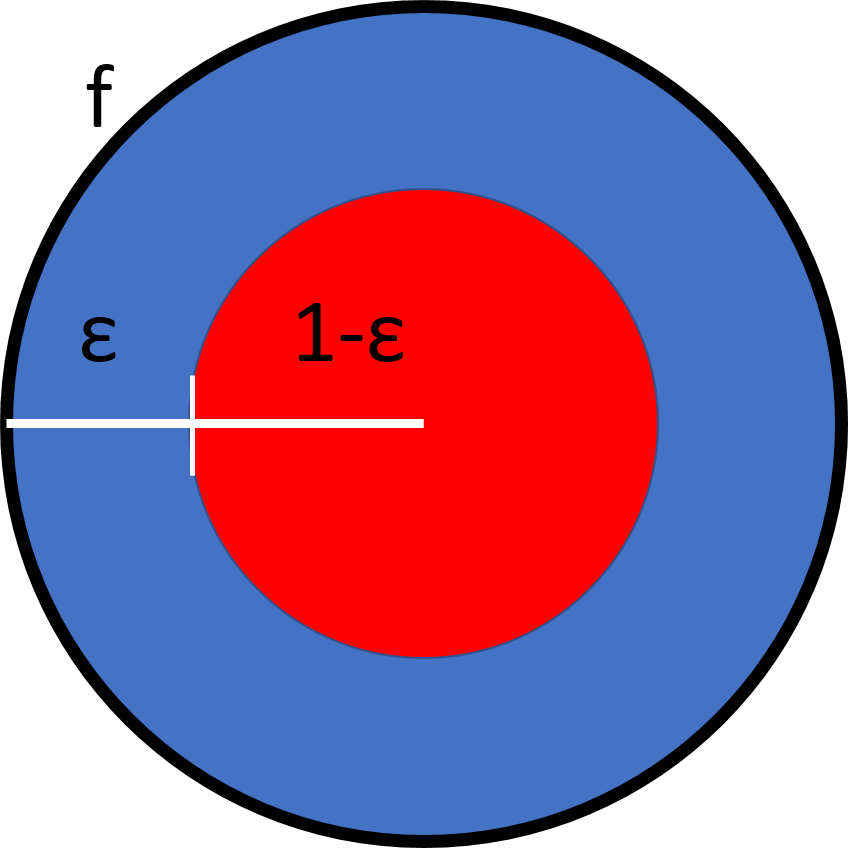
\includegraphics[width=0.7\linewidth]{Bild1}
\end{figure}



\end{document}
